\subsection{Procedury Składowane}

Zostały stworzone następujące procedury:
\begin{itemize}
	\item \href{run:Sources/SQL/6. Procedury Składowamne/032_Utworzenie_procedury_skladowanej_do_tworzenia_uzytkownikow.sql}{\texttt{utworz\_uzytkownika} - Procedura do tworzenia użytkowników}
\end{itemize}

\subsubsection{\texttt{utworz\_uzytkownika} - Procedura do tworzenia użytkowników}

Procedura ta służy do tworzenia użytkowników bazy SQL Server i dodawania ich do tabeli \texttt{uzytkownicy}.

Procedura przyjmuje 8 parametrów:
\begin{itemize}
	\item `@login VARCHAR(75)`
	\item `@nazwisko VARCHAR(75)`
	\item `@imie VARCHAR(75)`
	\item `@wiek INT`
	\item `@adres VARCHAR(150)`
	\item `@telefon VARCHAR(30)`
	\item `@plec CHAR(1)`
	\item `@haslo VARCHAR(30)`
\end{itemize}

Procedura zwraca następujące wartości:
\begin{itemize}
	\item 0 - Użytkownik dodany pomyślnie
	\item 1 - Wystąpił nieznany błąd
	\item 2 - Taki użytkownik już istnieje
\end{itemize}

\begin{lstlisting}[language=SQL, caption={Skrypt tworzący procedurę składowaną \texttt{utworz\_uzytkownika}}, label={lst:procedura-utworz_uzytkownika}]
CREATE PROCEDURE utworz_uzytkownika
  @login VARCHAR(75),
  @nazwisko VARCHAR(75),
  @imie VARCHAR(75),
  @wiek INT,
  @adres VARCHAR(150),
  @telefon VARCHAR(30),
  @plec CHAR(1),
  @haslo VARCHAR(30)
  AS
    IF EXISTS(SELECT * FROM uzytkownicy WHERE login = @login)
      RETURN 2;

    EXEC sp_addlogin @login, @haslo;
    EXEC sp_adduser @login;
    EXEC sp_addrolemember 'uzytkownicy_systemu', @login;

    BEGIN TRANSACTION;

    INSERT INTO uzytkownicy (login, nazwisko, imie, wiek, adres, telefon, plec)
      VALUES (@login, @nazwisko, @imie, @wiek, @adres, @telefon, @plec);

    IF @@ERROR<>0
      GOTO BLAD;

    COMMIT TRANSACTION
    RETURN 0;

    BLAD:
      ROLLBACK TRANSACTION
      RETURN 1;
\end{lstlisting}

\begin{figure}[h]
	\centering
    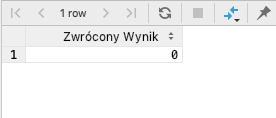
\includegraphics[width=0.25\textwidth]{procedura-utworz_uzytkownika-przyklad}
	\caption{Wynik prawidłowego uruchomienia przykładu użycia procedury \texttt{utworz\_uzytkownika}}
	\label{fig:lista_niepopularnych_obiektow}
\end{figure}

\begin{lstlisting}[language=SQL, caption={Przykład użycia procedury \texttt{utworz\_uzytkownika}}, label={lst:procedura-utworz_uzytkownika-przyklad}]
DECLARE @wynik INT;
EXEC @wynik = utworz_uzytkownika
  @login = 'j_kowalski',
  @nazwisko = 'Jan',
  @imie = 'Kowalski',
  @wiek = 25,
  @adres = 'Ul. Kowalska 23, 02-001, Warszawa',
  @telefon = '+48 625 548 874',
  @plec = 'M',
  @haslo = 'yourStrong(!)Password';
SELECT 'Zwrócony Wynik' = @wynik;
\end{lstlisting}